%----------------------------------------------------------------------------------------
% Proposta di progetto
%----------------------------------------------------------------------------------------

\documentclass[10pt]{softeng} % Document font size and equations flushed left

%----------------------------------------------------------------------------------------
%	DOCUMENT INFORMATION
%----------------------------------------------------------------------------------------

\Phase{Proposta di progetto}

\DocumentTitle{Proposta di progetto} % Document title

%----------------------------------------------------------------------------------------

\begin{document}

\startofdocument{}

\section{Visione del sistema}

Si vuole realizzare un sistema di Home Banking rivolto a persone fisiche (retail banking).
Considerata la necessit\`a crescente di aumentare la trasparenza bancaria e i controlli fiscali automatizzati, il governo ha varato\footnote{Quanto segue non rispecchia interamente la realt\`a.} un pacchetto di leggi che impone alle societ\`a di credito italiane di adeguarsi allo standard OBP \cite{obp} gi\`a in uso in Germania e nel Regno Unito \cite{obpuk}.
In questo contesto di transizione, la nostra societ\`a si propone di progettare un'applicazione che faccia da front-end per una banca che abbia adottato lo standard OBP.
La presenza di un'interfaccia unificata permetter\`a il \emph{deployment} del software presso pi\`u banche con minimo sforzo.

OBP \`e fondamentalmente un metodo standardizzato di accesso ai dati contenuti nel back-end della banca.
Nel momento in cui si adegua allo standard, ogni banca mantiene inalterate la struttura del suo database e dei sistemi preesistenti atti alla gestione delle operazioni bancarie.
Il software di OBP agisce quindi da \emph{wrapper} del sistema preesistente, mascherando completamente e rendendo inaccessibili le interfacce del back-end, ed esponendo all'esterno unicamente le interfacce definite dallo standard.
%Poich\'e l'introduzione del software OBP render\`a obsoleto eventuale software di Home Banking preesistente.

In figura \ref{fig:project_structure} \`e rappresentata informalmente la distribuzione di responsabilit\`a all'interno di una generica banca che adotti la nostra soluzione software.

La nostra applicazione permetter\`a ai clienti di effettuare le normali operazioni bancarie da casa, accedendo al sito della banca tramite web browser.

Il nostro sistema dovr\`a:
\begin{enumerate}
	\item Permettere la registrazione online di nuovi clienti.
		La registrazione deve essere ultimata presso una filiale della banca.
	\item Utilizzare lo standard TOTP \cite{totprfc}.
	\item Permettere all'utente di effettuare le seguenti operzioni:
		\begin{enumerate}
			\item visualizzare il saldo (contabile, disponibile e liquido)
			\item visualizzare lo storico delle transazioni effettuate
			\item gestire le proprie carte di credito e carte prepagate
			\item disporre pagamenti di vario tipo (bonifici ordinari, bonifici SEPA, ricariche prepagate, ricariche telefoniche, pagamenti bollettini, etc)
			\item gestire portafogli fondi, azioni, obbligazioni e titoli statali % TODO CHECK SYNTAX
		\end{enumerate}
	\item Permette di effettuare l'audit di sicurezza agli addetti della banca.
	\item Notificare all'utente (tramite SMS e/o email) determinati eventi.
\end{enumerate}

Simuleremo la realizzazione del progetto seguendo lo Unified Process, producendo la documentazione richiesta da ogni iterazione e flusso di lavoro.
L'implementazione del sistema non \`e coperta dal progetto.

\section{Documentazione}

La documentazione che produrremo comprender\`a:
\begin{enumerate}
	\item Studio di fattibilit\`a e analisi del contesto.
	\item Specifica dei requisiti e modello di business.
	\item Documento di analisi dei rischi.
	\item Bozza di contratto per il cliente (basata sulla specifica dei requisiti prodotta).
	\item Analisi e progetto del sistema secondo le modalit\`a richieste (schede CRC, analisi nomi/verbi, classi di analisi e classi di progetto, casi d'uso).
	\item Analisi dei costi e pianificazione temporale.
	\item Piano dei test.
\end{enumerate}
L'ordinamento dei documenti non \`e vincolante, ma \`e stato comunque scelto coscientemente.
In particolare l'analisi dei rischi verr\`a fatta prima di redigere la bozza di contratto, poich\'e il sistema che intendiamo sviluppare ha forti requisiti di sicurezza, ed \`e opportuno conoscere i rischi gi\`a nelle fasi iniziali del processo software.

%----------------------------------------------------------------------------------------
%	REFERENCE LIST
%----------------------------------------------------------------------------------------

\printcustombib{} 

%----------------------------------------------------------------------------------------
%	FIGURES
%----------------------------------------------------------------------------------------

\graphicspath{{Images/}}
\begin{figure*}[hbt]
	\centering
	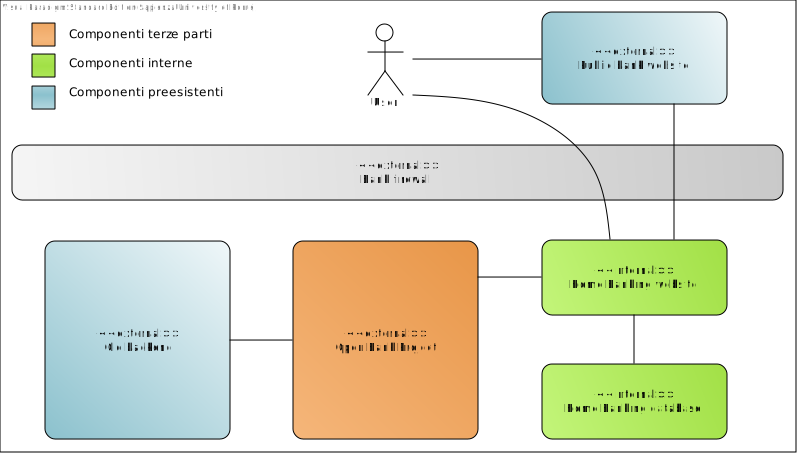
\includegraphics[width=\textwidth]{architettura_sistema}
	\caption{Proposta architetturale ad alto livello della struttura del progetto.}
	\label{fig:project_structure}
\end{figure*}

\begin{figure*}[tp]
	\centering
	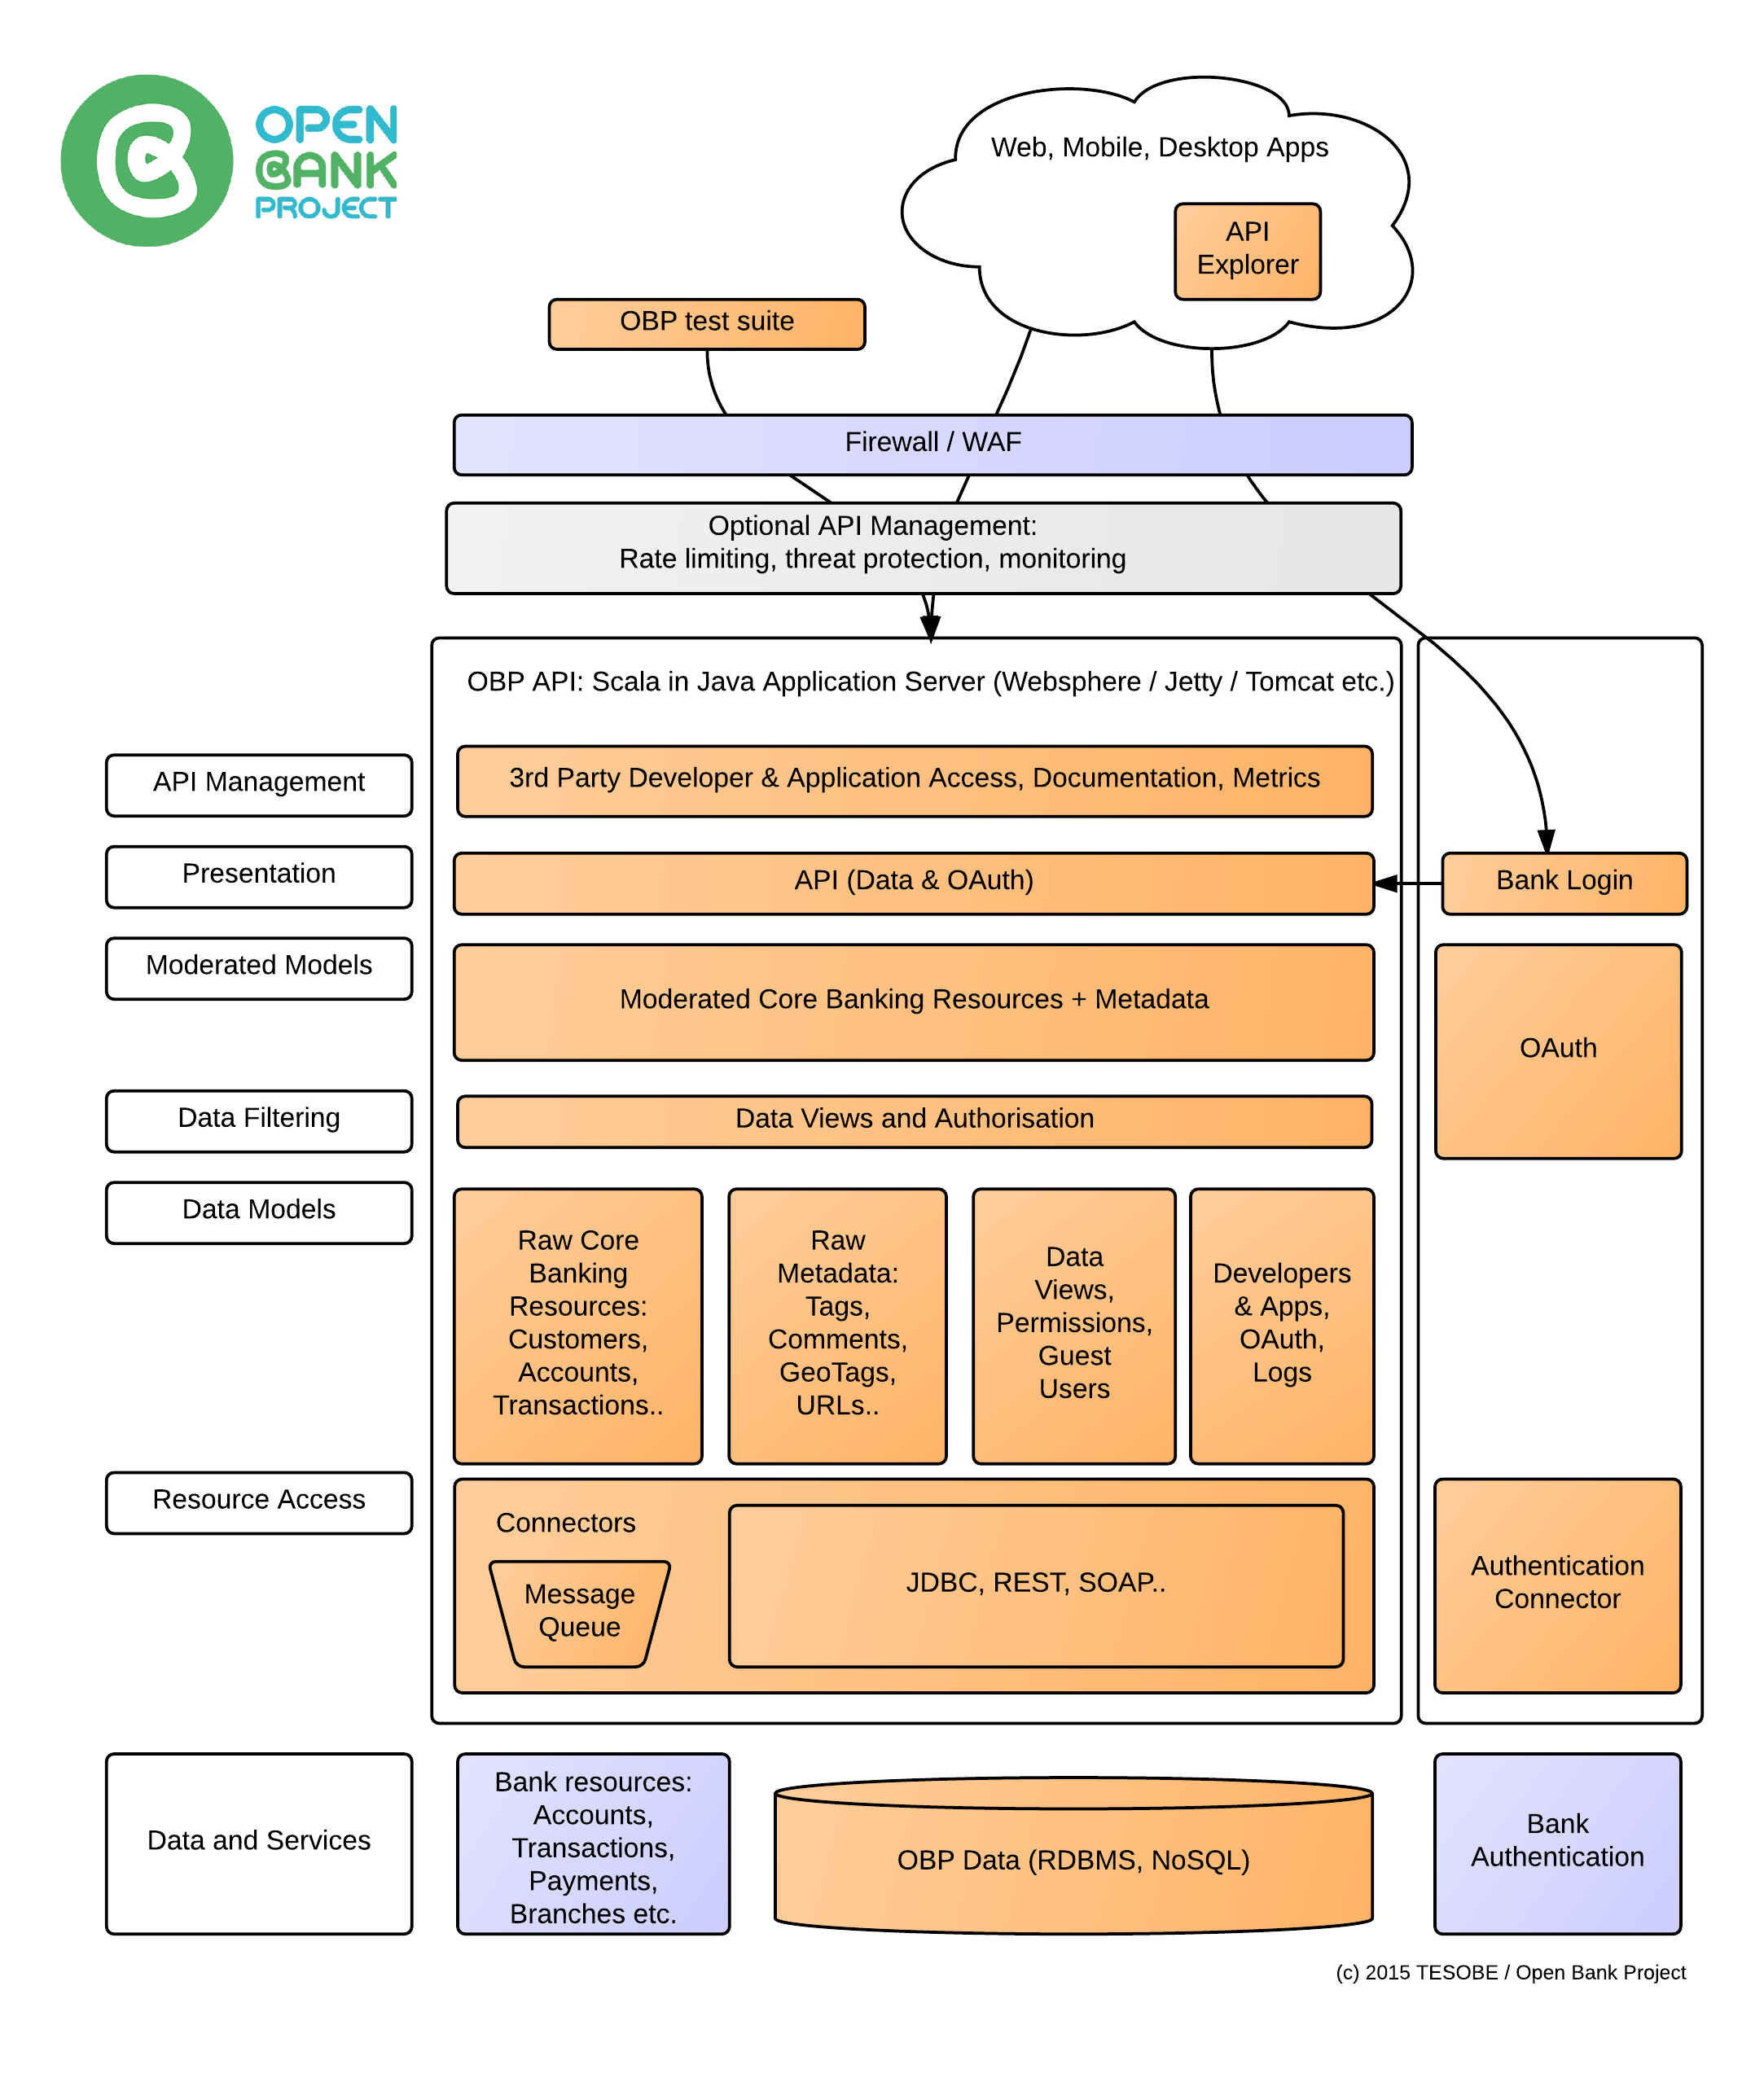
\includegraphics[width=\textwidth]{open_bank_project_architecture}
	\caption{Architettura del software di Open Bank Project\cite{obparch}.}
	\label{fig:open_bank_project_architecture}
\end{figure*}

\begin{figure*}[hbt]
	\centering
	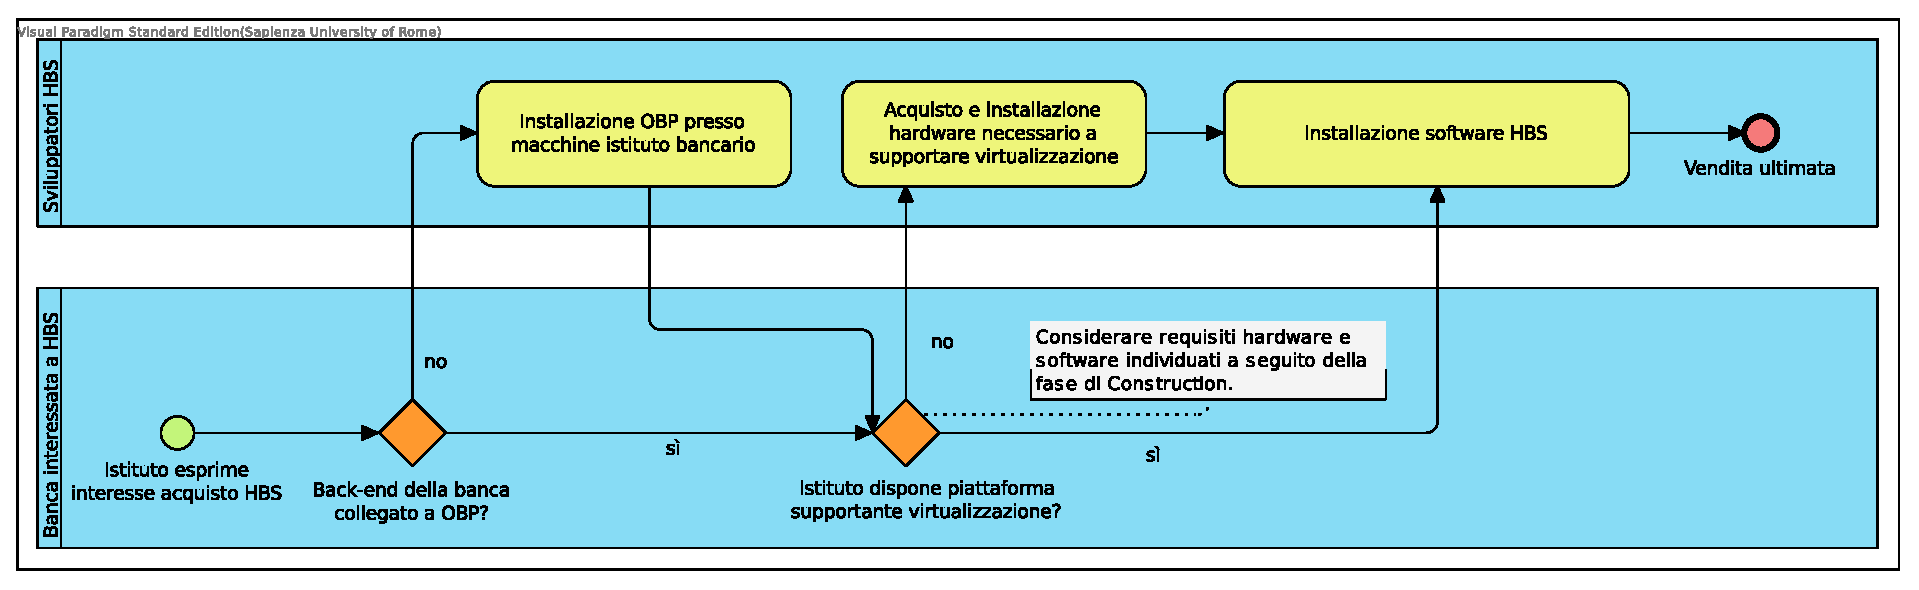
\includegraphics[width=\textheight, angle=90]{Images/Home_Banking_software_sale.eps}
	\caption{Business case: vendita software sviluppato a clienti finali.}
	\label{fig:business_case_vendita_software}
\end{figure*}

\end{document}

